% !TeX spellcheck = da_DK
% Setup document class.
%  This will always be the beamer class, but depending on the use of notes,
%  it can be annotated with the option [notes] or  [notes=only], depending
%  on whether notes should be included, or should be the only thing in
%  the document.
\documentclass{beamer}

% Setup theme.
%\usetheme[
%%% options passed to the outer theme
%    progressstyle=fixedCircCnt,   %either fixedCircCnt, movCircCnt, or corner
%    rotationcw,          % change the rotation direction from counter-clockwise to clockwise
%    shownavsym          % show the navigation symbols
]{AAUsimple}

\usetheme[
%%% options passed to the outer theme
%    hidetitle,           % hide the (short) title in the sidebar
%    hideauthor,          % hide the (short) author in the sidebar
%    hideinstitute,       % hide the (short) institute in the bottom of the sidebar
%    shownavsym,          % show the navigation symbols
%    width=2cm,           % width of the sidebar (default is 2 cm)
    hideothersubsections,% hide all subsections but the subsections in the current section
%    hideallsubsections,  % hide all subsections
    left               % right of left position of sidebar (default is right)
%%% options passed to the color theme
%    lightheaderbg,       % use a light header background
  ]{AAUsidebar}



% Import preamble
%%% Initial things %%%
% Increase number of dimen registers
\usepackage{etex}
% Fix various issues with LaTeX2e
\usepackage{fixltx2e}
% Font package
\usepackage{fourier}


%%% Translations and character encodings %%%
% Enable use of several characters, including æ, ø and å
\usepackage[utf8]{inputenc}
% Danish language
\usepackage[danish]{babel}
% Use PostScript fonts instead of bitmap ones. Also does other stuff.
\usepackage[T1]{fontenc}
% Various LaTeX symbols
\usepackage{latexsym}
% Wider selection of colours
\usepackage{xcolor}
% Improved element justification
\usepackage{ragged2e}
% Font improvements
\usepackage{fix-cm}
% Enables various forms of lines, like double-underlining (\uuline{})
\usepackage{ulem}
% Sets the tolerance for distance between words, determining when to hyphenate.
\pretolerance=2500


%%% Figures and tables (Floats) %%%
% Enable multi-rows and -columns
\usepackage{multirow}
\usepackage{multicol}
% Double, horizontal lines
\usepackage{hhline}
% Enables coloured tables
\usepackage{colortbl}
% Prettier tables
\usepackage{booktabs}


%%% Mathematic formulas %%%
% AMS math
\usepackage{amsmath}
\usepackage{amssymb}
% Extra fonts (for math, I think)
\usepackage{stmaryrd}
% Access text symbols
\usepackage{textcomp}
% Extend AMS
\usepackage{mathtools}
\usepackage{cancel}


%%% Graphics %%%
% Various image-commands
\usepackage{eso-pic}
% Use JPEG and PNG images
\usepackage{graphicx}


%%% References, bibtex and URLs %%%
% Post URLs. Allows breaking at hyphens to help avoid long links.
\usepackage{url}
% Better cross references
\usepackage[danish]{varioref}
% Define a new 'leo' style for URL package, that will use a smaller font
\makeatletter
\def\url@leostyle{%
  \@ifundefined{selectfont}{\def\UrlFont{\sf}}{\def\UrlFont{\small\ttfamily}}
}
\makeatother
% And of course, use this new style
\urlstyle{leo}

\hypersetup{pdfstartview={Fit}}

% Define document stuff
\title[Sejlklubadministration]{Bådudlån i sejlklubber}
\subtitle[Statusseminar]{Statusseminar}
\author[SW2A305]{Gruppe SW2A305}
\date{10. marts 2014}

\institute[
%  {\includegraphics[scale=0.2]{aau_segl}}\\ %insert a company, department or university logo
Første Studieår (Software)\\
Aalborg Universitet\\
Danmark
] % optional - is placed in the bottom of the sidebar on every slide
{% is placed on the title page
  Første Studieår --- Software\\
  Aalborg Universitet\\
  Danmark
  
  %there must be an empty line above this line - otherwise some unwanted space is added between the university and the country (I do not know why;( )
}

% Specify a logo on the titlepage (you can specify additional logos an include them in 
% institute command below
\pgfdeclareimage[height=1.5cm]{titlepagelogo}{AAUgraphics/aau_logo_new} % placed on the title page
%\pgfdeclareimage[height=1.5cm]{titlepagelogo2}{graphics/aau_logo_new} % placed on the title page
\titlegraphic{% is placed on the bottom of the title page
  \pgfuseimage{titlepagelogo}
  %  \hspace{1cm}\pgfuseimage{titlepagelogo2}
}


\begin{document}

{\aauwavesbg
  \begin{frame}[plain,noframenumbering]
    \titlepage
  \end{frame}}

% ==================== SUBJECTS ======================
%% !TeX spellcheck = da_DK
\section{Section 1}

% === Slide: Title ===
\begin{frame}{Title of frame}

\structure{This is part of the structure.}

\vspace{2mm}

This is some text\ldots

\note{This is a note}

\begin{itemize}
  \item First point
  \item Second point
\end{itemize}

\note{Another note here\ldots}

\end{frame}

% --- Subsection name ---
\subsection{Subsection 1}

% === Slide: Another title ===
\begin{frame}{Another title}

Wee!

\end{frame}

\section{Program Demonstration}

\begin{frame}{Program demonstration}
	
	\begin{itemize}
		\item Database 
		\item Hvad sker der ved opstart?
		\item Hvad sker der når programmet lukkes?
	\end{itemize}

	
\end{frame}
\section{Interessenter}
\begin{frame}{Interessenter}
	\framesubtitle{Analyse af interessenterne}
	
	\begin{itemize}
		\item Fritidsklubber
		\item Sportsklubber
		\begin{itemize}
			\item Medlemshåndtering og betaling
			\item Holde styr på baner
			\item Holdopbygning og taktik
		\end{itemize}
		\item Skydning
		\item Golf
		\item Haller
		\begin{itemize}
			\item Adminstration af baner og omklædning
			\item Informationsdeling
			\item Adminstration af kiosk	
		\end{itemize}
		\item Netcaféer
		\item Sejlklubber
	\end{itemize}


\end{frame}

\section{Organisation}
\begin{frame}{Organisation}
	\framesubtitle{Analyse af organisationen}
		\begin{itemize}
			\item Interessenter for sejlklubbers administrative opgaver
			\begin{itemize}
				\item Dansk Sejlunion
				\item Medlemmer
				\item Undervisere
			\end{itemize}
			\item Research af klubber
			\begin{itemize}
				\item Sejlklubben Sundet
				\item Andre sejlklubber
			\end{itemize}
		\end{itemize}

\end{frame}

\section{Datalag}

\definecolor{positivegreen}{rgb}{0,0.7,0}
\definecolor{negativeyellow}{rgb}{0.8,0.8,0}
\definecolor{badred}{rgb}{0.8,0,0}


\subsection{Modellag}

\begin{frame}{Modellag}
  \framesubtitle{Umm\ldots}
  \begin{itemize}
    \item<1-> What to put here\ldots
  \end{itemize}
\end{frame}


\subsection{Persistenslag}

\begin{frame}{Persistenslag}
  \framesubtitle{Entity Framework --- Code First}
  \begin{itemize}
    \item<1-> \color{positivegreen}Isolering af databaselogik (SQL--forespørgsler)
    \item<1-> \color{positivegreen}POCO (Plain Old CLR Objects)
    \item<1-> \color{positivegreen}RAD (Rapid Application Development)
    \item<2-> \color{negativeyellow}Migrations
    \item<2-> \color{negativeyellow}Data Annotations
    \item<3-> \color{badred}Context levetid
  \end{itemize}
\end{frame}

\begin{frame}{Persistenslag}
  \framesubtitle{SQLite}
  \begin{itemize}
    \item<1-> \color{positivegreen}Kræver kendskab til SQL.
    \item<1-> \color{positivegreen}Komplekse relationer kan være svære.
    \item<1-> \color{negativeyellow}Fuld kontrol over det underliggende.
    \item<2-> \color{negativeyellow}Enkeltbrugersystem --- Ikke thread--safe.
    \item<3-> \color{badred}''Database is locked``
  \end{itemize}
\end{frame}

\begin{frame}{Persistenslag}
  \framesubtitle{Mock--data med persistens}
  \begin{itemize}
    \item<1-> \color{positivegreen}Hurtigt --- Hukommelsesbaseret.
    \item<1-> \color{negativeyellow}Ikke skalerbart.
    \item<1-> \color{negativeyellow}Risiko for datatab.
  \end{itemize}
\end{frame}
\section{Datalag}
\subsection{Teknologianalyse}

\begin{frame}{Teknologianalyse}
  \begin{itemize}
    \item BoatCloud
    \begin{itemize}
      \item StackTrack
      \item VesselValet
      \item TicketTracker
    \end{itemize}
    \item SailingClubManager
    \begin{itemize}
      \item Sejlklubsbaseret
    \end{itemize}
    \item ForeningLet
    \begin{itemize}
      \item Generelt for fritidsklubber
    \end{itemize}
  \end{itemize}
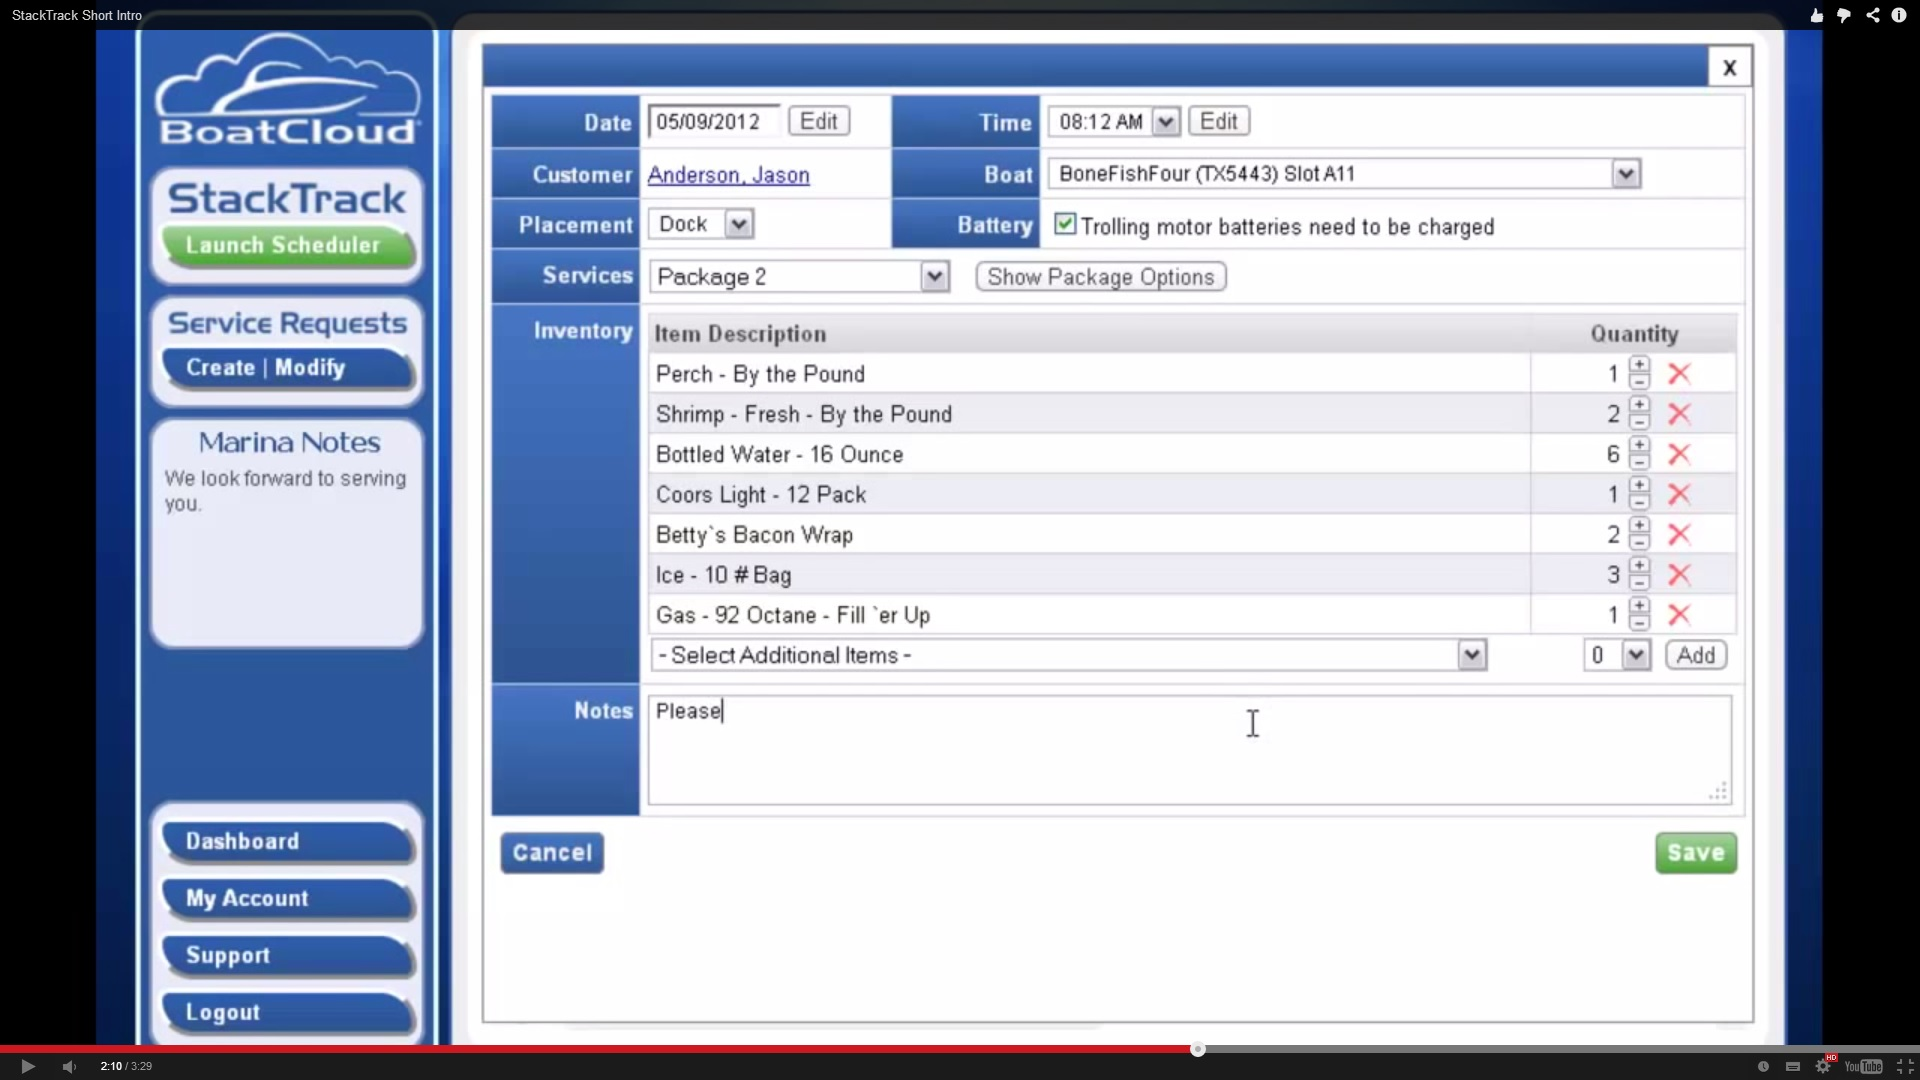
\includegraphics[width=0.5\textwidth]{images/StackTrack.jpg}
\end{frame}

\begin{frame}{Teknologianalyse}
  \begin{itemize}
    \item BoatCloud
    \begin{itemize}
      \item StackTrack
      \item VesselValet
      \item TicketTracker
    \end{itemize}
    \item SailingClubManager
    \begin{itemize}
      \item Sejlklubsbaseret
    \end{itemize}
    \item ForeningLet
    \begin{itemize}
      \item Generelt for fritidsklubber
    \end{itemize}
  \end{itemize}
  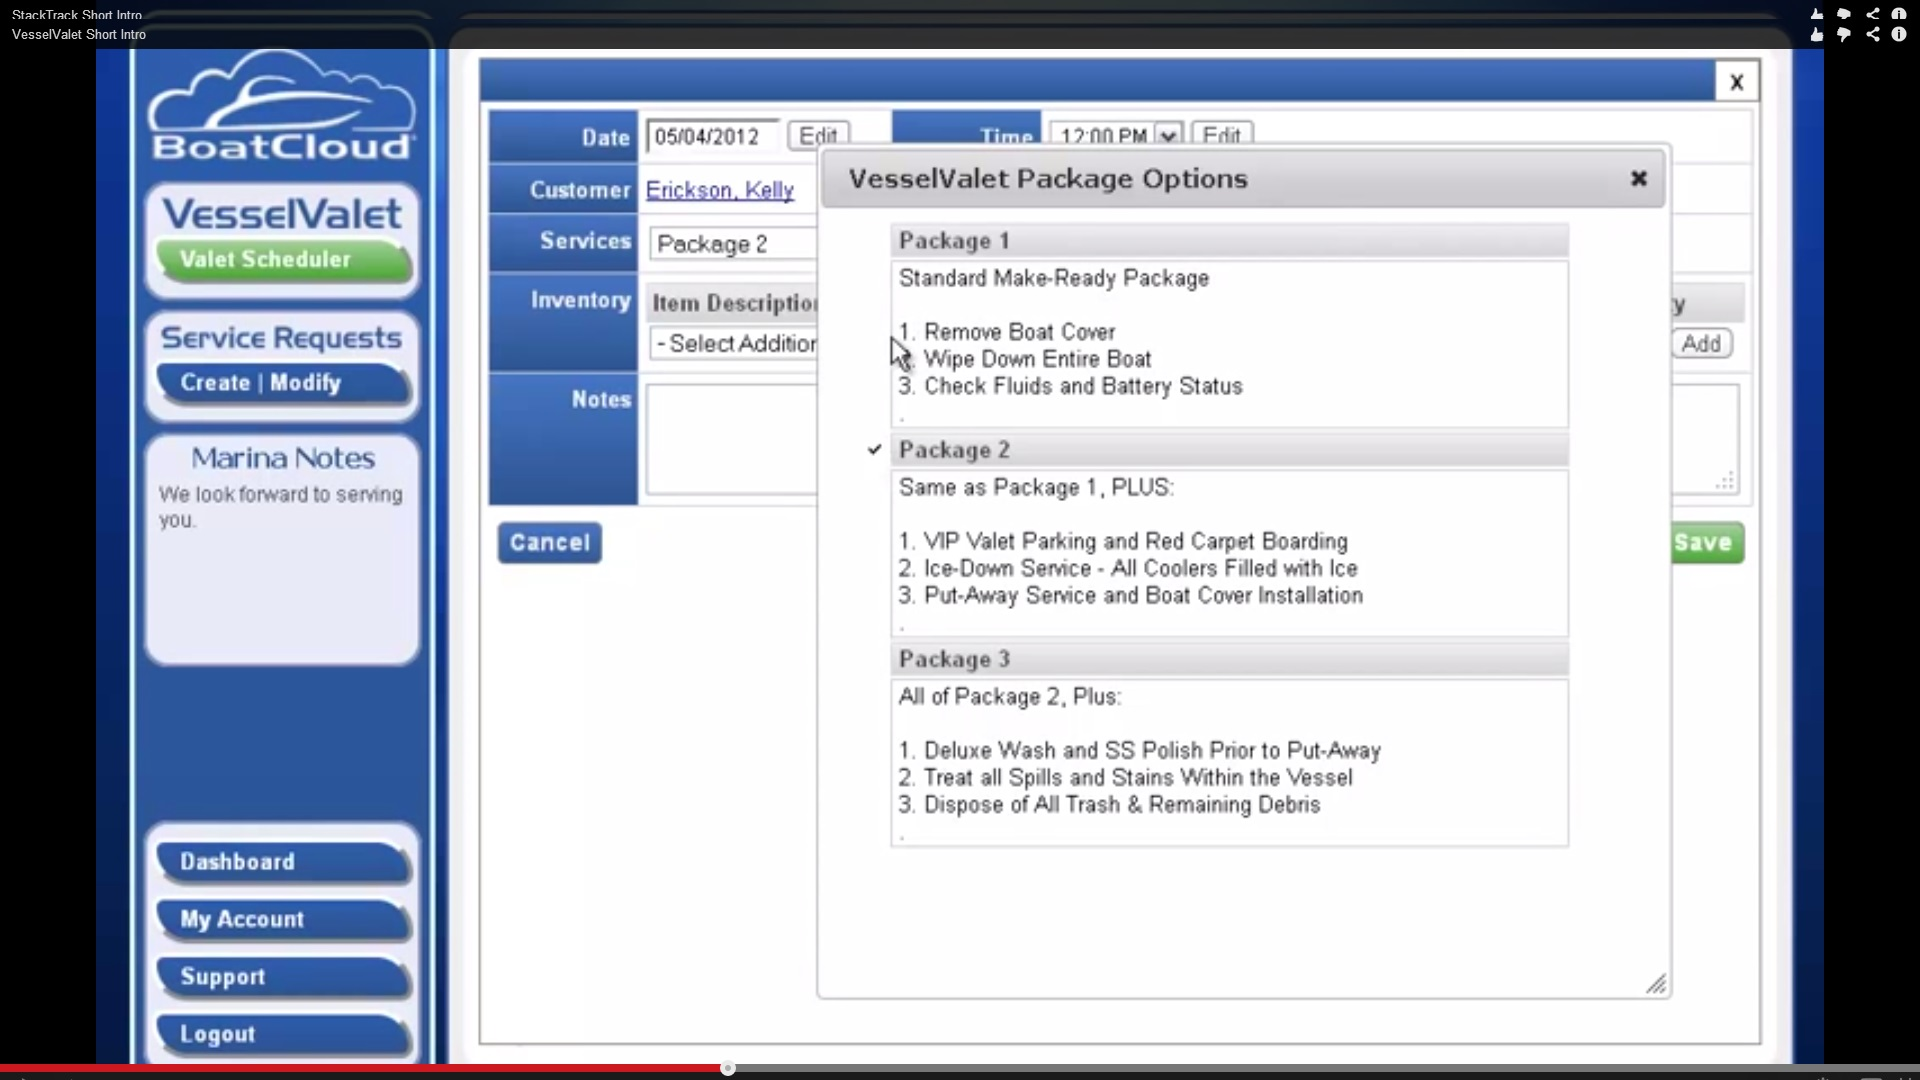
\includegraphics[width=0.5\textwidth]{images/VesselValet.jpg}
\end{frame}

\begin{frame}{Teknologianalyse}
  \begin{itemize}
    \item BoatCloud
    \begin{itemize}
      \item StackTrack
      \item VesselValet
      \item TicketTracker
    \end{itemize}
    \item SailingClubManager
    \begin{itemize}
      \item Sejlklubsbaseret
    \end{itemize}
    \item ForeningLet
    \begin{itemize}
      \item Generelt for fritidsklubber
    \end{itemize}
  \end{itemize}
  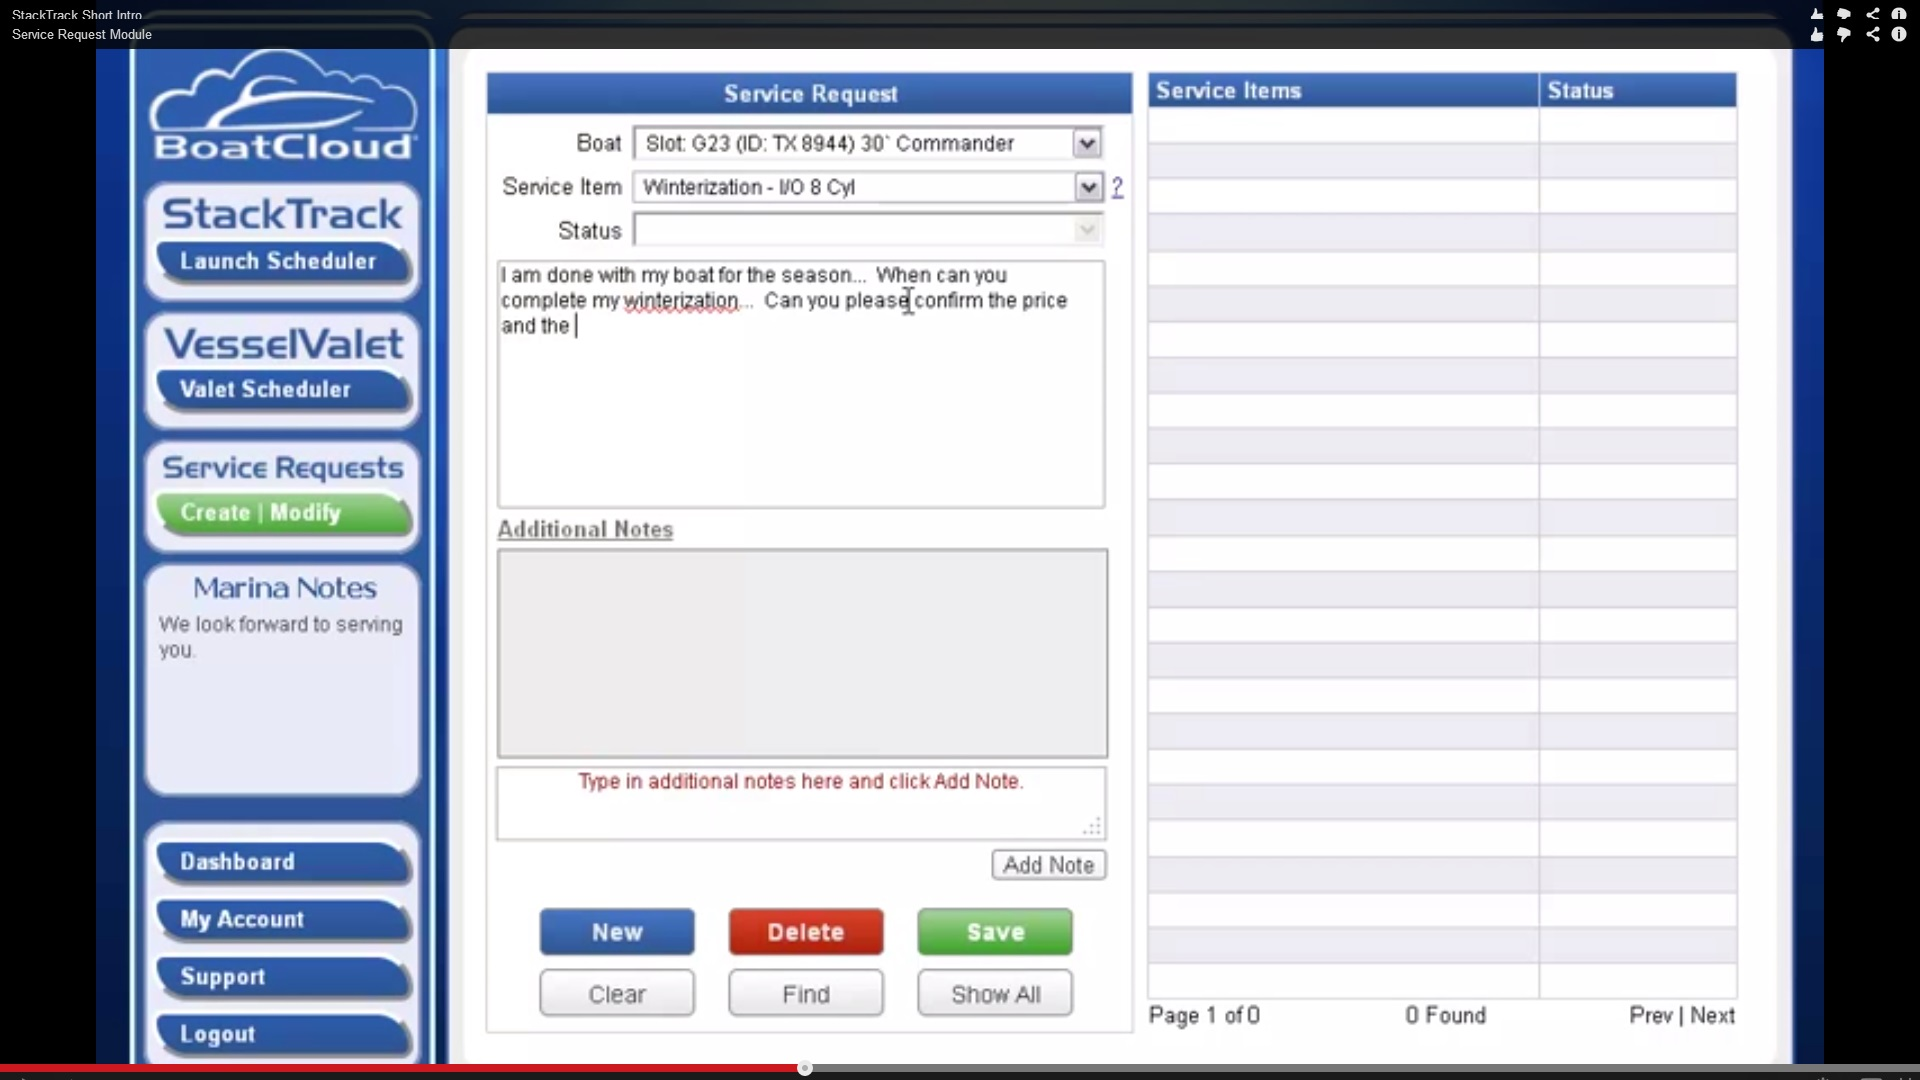
\includegraphics[width=0.5\textwidth]{images/TicketTracker.jpg}
\end{frame}

\begin{frame}{Teknologianalyse}
  \begin{itemize}
    \item BoatCloud
    \begin{itemize}
      \item StackTrack
      \item VesselValet
      \item TicketTracker
    \end{itemize}
    \item SailingClubManager
    \begin{itemize}
      \item Sejlklubsbaseret
    \end{itemize}
    \item ForeningLet
    \begin{itemize}
      \item Generelt for fritidsklubber
    \end{itemize}
  \end{itemize}

\end{frame}

\begin{frame}{Teknologianalyse}
  \begin{itemize}
    \item BoatCloud
    \begin{itemize}
      \item StackTrack
      \item VesselValet
      \item TicketTracker
    \end{itemize}
    \item SailingClubManager
    \begin{itemize}
      \item Sejlklubsbaseret
    \end{itemize}
    \item ForeningLet
    \begin{itemize}
      \item Generelt for fritidsklubber
    \end{itemize}
  \end{itemize}
  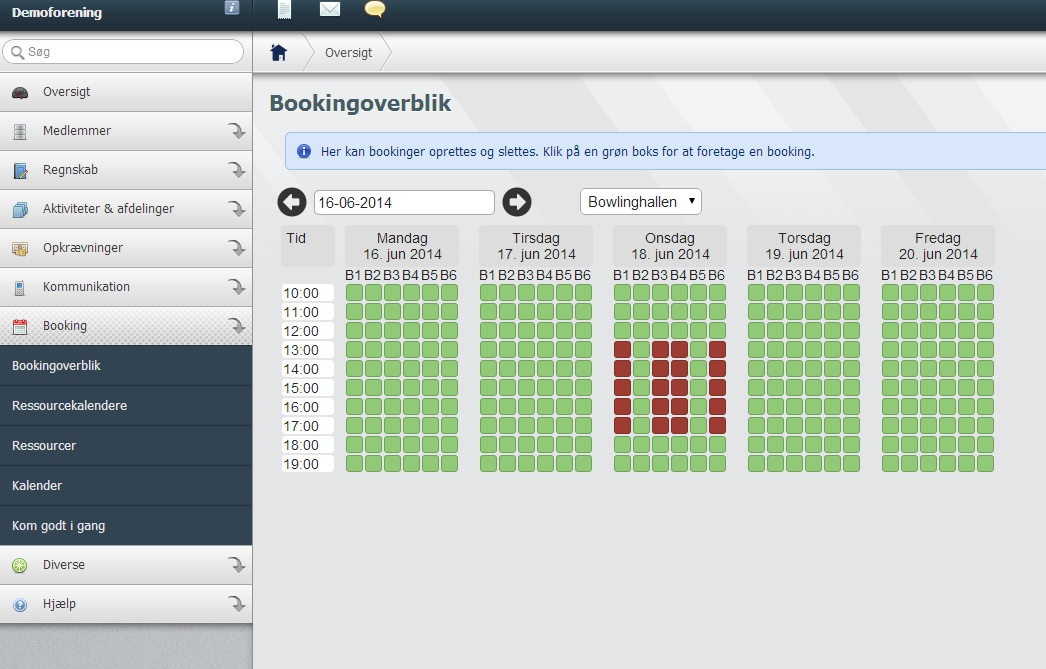
\includegraphics[width=0.5\textwidth]{images/ForeningLet.jpg}
\end{frame}


\subsection{Problemformulering}

\begin{frame}{Problemformulering}
  \begin{itemize}
    \item Det er et problem at frivillige i fritidsklubber med specielle udlejningsmuligheder, så som Sejlklubben Sundet, benytter unødvendig arbejdskraft på fysisk dokumenthåndtering vedrørende udlånte faciliteter, undervisning og begivenhedsorganisation. Hvordan kan der udvikles et system som kan hjælpe med at danne overblik over sådanne opgaver?
    \item Hvilke informationer ville et sådan system skulle holde styr på?
    \item Er det muligt at arbejde sammen med systemer allerede I brug ved klubben?
    \item Hvordan skal et sådan system arrangeres for at gøre det let at bruge?
  \end{itemize}
\end{frame}
\section{Introduktion}

\begin{frame}{Introduktion}
\framesubtitle{Disposition}
	\begin{itemize}
	\item Introduktion (Nikolaj)
	\item SOTA, problemformulering og udviklingsproces (Marc)
	\item Produktkrav og programopbygning
	
	
	\end{itemize}

\end{frame}

\begin{frame}{Introduktion}
	\begin{itemize}	
	\item Valg af projektforslag
	\item Initierende problem			
	\newline
		
		\begin{tabular}{|p{8cm}|}
		\textit{Er det muligt at lave en softwareløsning, der kan gøre frivillige i fritidsklubbers administrative
		arbejde nemmere, som stadig er let at benytte uden at have meget erfaring med anvendelse af computersystemer, og i så fald hvordan?}
  		\end{tabular}
	\end{itemize}
\end{frame}


\section{Sejlklubben Sundet}

\begin{frame}{Sejlklubben Sundet}

	\begin{itemize}
	\item Afgrænsning til Sejlklubben Sundet
			\begin{itemize}
			\item Vestre Bådlaug interviewet og andre klubber kontaktet
			\end{itemize}
	\item Mere information til rådighed
			\begin{itemize}
			\item Jacob - Tidligere skolechef
			\item Hjemmeside
			\end{itemize} 
	\item Konkrete funktioner
		\begin{itemize}
		\item Undervisningshåndtering
		\item Bådudlån
		\item Begivenhedsinformation og tilmelding
		\end{itemize}
	
	\end{itemize}
	
\end{frame}
% ====================================================

% Final slide
{\aauwavesbg
  \begin{frame}[plain,noframenumbering]
    \finalpage{\texttt{\textbf{return} 0;}}
  \end{frame}}

\end{document}
